\documentclass[12pt]{article}
\usepackage{graphicx} % Required for inserting images
\usepackage{enumitem}
\usepackage{amsmath}
\usepackage{gvv-book}
\usepackage{gvv}

\title{\textbf{1.4.19}}
\author{\textbf{EE25BTECH11004 - Aditya Appana}}
\date{August 26, 2025}

\begin{document}

\maketitle

\section*{Question}
Find a point on the X axis, which is equidistant from the points 
\begin{align*}
\myvec{ 7 \\ 6 }\text{ and }\myvec{3 \\ 4}
\end{align*}

\section*{Solution}
Let vectors be 
\begin{align} 
\vec{P}=\myvec{7 \\ 6} \\
\vec{Q}=\myvec{3 \\ 4}
\end{align}

\vspace{1cm}

We need to find the point $\vec{R}$ on the X-axis which is equidistant from $\vec{P}$ and $\vec{Q}$ \\
The formula to calculate the x-coordinate of the point $\vec{R}$ is

\vspace{1cm}


$$x= \frac{ ||\mathbf{P}||^2 - ||\mathbf{Q}||^2 }{2\mathbf{(P-Q)^T e_1}}$$


\vspace{1cm}

\newpage
Substituting $\mathbf{P, Q}$, and $e_1$ in this formula :


$$x = \frac{7^2+6^2-(3^2+4^2)}{2 \myvec{4 \\ 2}^T \myvec{1\\0}}$$


$$=\frac{60}{8}$$



$$= 7.5$$ \\





Therefore, the required point is (7.5,0)

\begin{figure}[H]
    \centering
    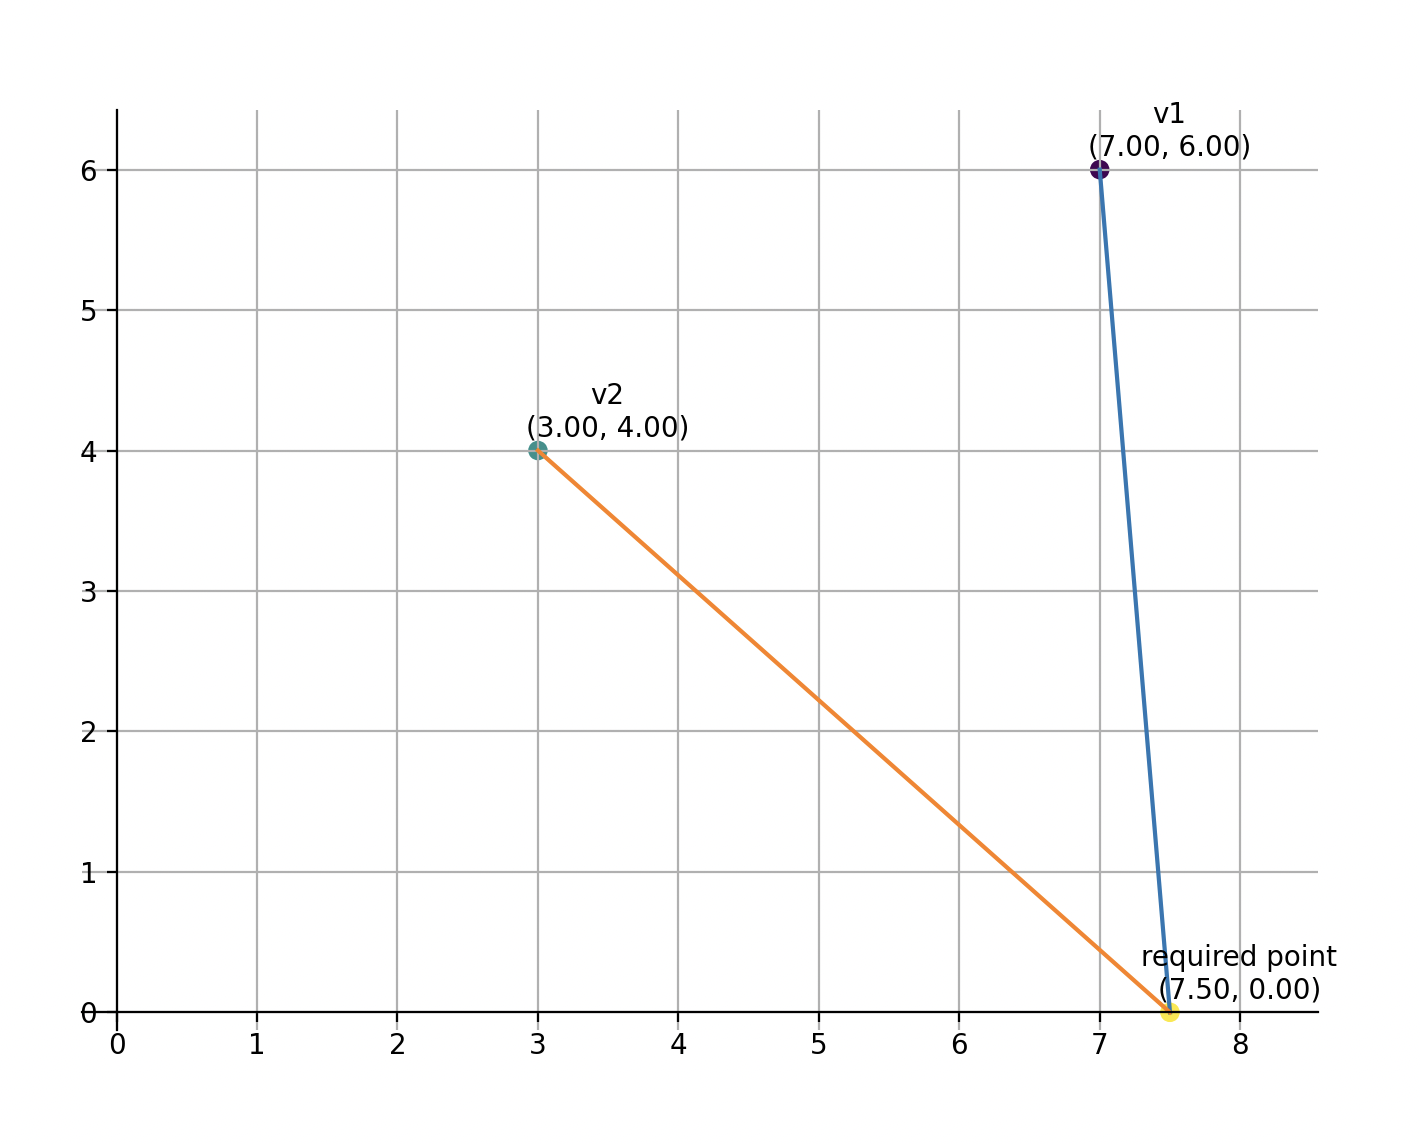
\includegraphics[width=1.0\columnwidth]{Figs/Figure_2.png}
    \caption{Plot}
    \label{fig:placeholder}
\end{figure}
\end{document}